\section{Aufgabe I}

\begin{figure}[h!]
    \centering
    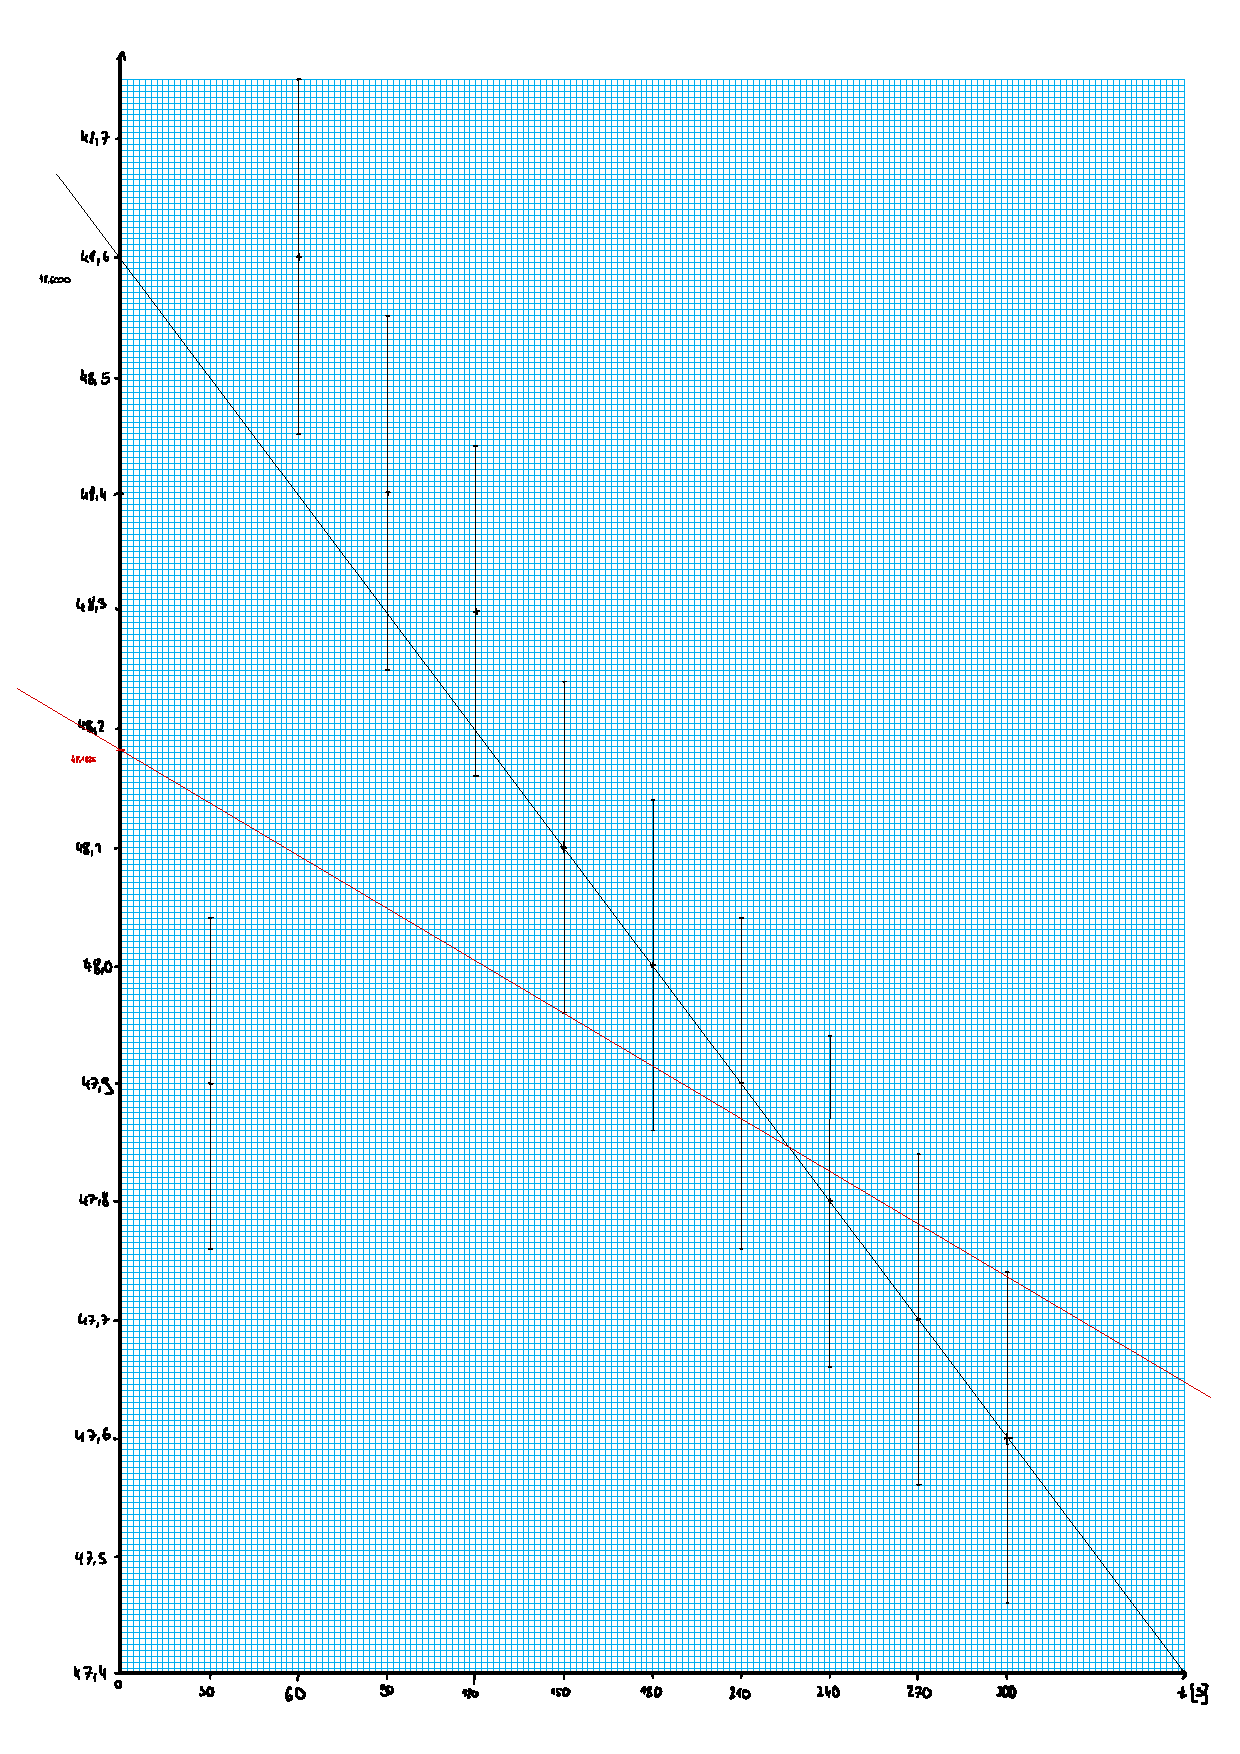
\includegraphics[page=1, width=0.95\textwidth,]{Verusch42Dia.pdf}
    \caption{Diagramm 1}
\end{figure}
\newpage

In Diagramm 1 wurden die gemessenen Temperaturen im Kalorimeter gegen die vergangene Zeit aufgetragen. Die Werte
stammen aus Tabelle 2. Durch verlängerung des linearen Anteils zum Anfangszeitpunkt $t = 0s$ konnte die Gleichgewichtstemperatur$\overline{T}$ abgelesen werden.
Der Fehler wird mithilfe einer Fehlergeraden bestimmt. Durch die Differenz der Werte bei $t=0$ ergibt sich der Fehler:

\[ \underline{\underline{\overline{T} = (48,6 \pm 0,4)^\circ \text{C}}}\]

\begin{equation}
    \Delta \overline{T}= \overline{T}- \overline{T}_{Fehler}
\end{equation}

Aus der Gleichgewichtstemperatur $\overline{T}$ lässt sich die Wärmekapazität des Kalorimeter also der Wasserwert mit Gleichung \ref{eq:Wasserwert} berechnen:

\[\underline{\underline{W= ( 95 \pm  17)\ \tfrac{\text{J}}{\text{K}}}}\]
Der Fehler folgt nach dem Fehlerrechner aus dem Skript:
\begin{equation}
    \frac{\Delta W}{W}=\sqrt{\frac{\Delta T^{2} \left(T_{2} - T_{1} \right)^{2}}{\left(T - T_{1}\right)^{2} \left(T - T_{2}\right)^{2}} + \frac{\Delta T_{1}^{2}}{\left(T - T_{1}\right)^{2}} + \frac{\Delta T_{2}^{2}}{\left(T - T_{2}\right)^{2}} + \frac{\Delta m_{k}^{2}}{\left(m_{k} - m_{w}\right)^{2}} + \frac{\Delta m_{w}^{2}}{\left(m_{k} - m_{w}\right)^{2}} + \frac{\Delta c_{w}^{2}}{c_{w}^{2}}}
\end{equation}

Vergleicht man den erhaltenen Wert mit dem Literaturwert von $70 \ \tfrac{\text{J}}{\text{K}}$ so ergibt sich eine Abweichung des Messwerts von $1,5 \ \sigma$

\section{Aufgabe II}

Für die Berechnung der spezifischen Wärme muss zuerst die Siedetemperatur des Wassers bei gemessenem Luftdruck berechnet werden. Dabei gilt nach Gleichung \ref{eq:Siedetemperatur}
für die Siedetemperatur $T_1$ mit einem gemessen Luftdruck von $1012,3$hPa:

\[T_1 = (99,9806 \pm 0,0028) ^\circ \text{C}\]

Daraus ergibt sich für die speziefische Wärmekapazität $c_m$ nach Gleichung \ref{eq:KalC} und die Molwärme $c_{mol} = c_m\cdot M$ mit M als molarer Masse:

\begin{table}[h!]
    \centering
    \begin{tabular}{r r r r r r}
        \toprule
        Material & $m_{kw}[g]$& $T_{vor} [^\circ C] $&  $T_{nach}[^\circ C] $& $c_m$[J/gK] & $c_{mol}$[J/$mol$K] \\
        \midrule
        Graphit & $592,47 \pm 0,01 $ & $24,30 \pm 0,07$ & $28,70 \pm 0,09$ & $0,77 \pm 0,02 $ & $9,25\pm0,24$\\
        Alu. &$622,29 \pm 0,01$ &$30,6 \pm 0,1 $&$ 35,7 \pm0,1$& $0,84 \pm 0,03$ & $22,7 \pm 0,8$\\
        Blei & $ 623,28 \pm 0,01$ & $28,00 \pm 0,08$& $31,20 \pm 0,09$ & $0,13 \pm 0,01$ & $27 \pm 2$\\
        \bottomrule
        
    \end{tabular}
    \caption{Wärmekapazitäten gemessen im Kalorimeter}
\end{table}
Dadurch, dass beim Thermometer ein systematsicher Fehler vorhanden ist, wird zuerst die Differenz $A = \overline{T} - T_2$ berechnet, da sich dort dieser Fehler aufhebt.
Bei der restlichen Fehlerrechnung wurde der systematische Fehler berücksichtigt.
\begin{align}
    (\frac{\Delta c_m}{c_m})^2 &=\frac{c_{w}^{2} \Delta m_{k}^{2}}{\left(W - c_{w} m_{k} + c_{w} m_{w}\right)^{2}} + \frac{c_{w}^{2} \Delta m_{w}^{2}}{\left(W - c_{w} m_{k} + c_{w} m_{w}\right)^{2}} \notag \\
    & + \frac{\Delta T^{2}}{\left(T - T_{2}\right)^{2}} + \frac{\Delta T_{2}^{2}}{\left(T - T_{2}\right)^{2}} + \frac{\Delta W^{2}}{\left(W - c_{w} m_{k} + c_{w} m_{w}\right)^{2}}\notag \\
    & + \frac{\Delta c_{w}^{2} \left(m_{k} - m_{w}\right)^{2}}{\left(W - c_{w} m_{k} + c_{w} m_{w}\right)^{2}} + \frac{\Delta m_{x}^{2}}{m_{x}^{2}} + \frac{\Delta A^{2}}{A^{2}}\notag\\
\end{align}

\subsection{Vergleiche}
Die Werte werden nun mit den Literaturwerten Verglichen. Zusätzlich wird die speziefische Wärmekapazität
mithilfe Dulong-Petit berechnet:
\begin{equation}
    c_{DP} = 3 \frac{R}{M}
\end{equation}
Mit $R = 8,314 \frac{\text{J}}{mol \text{K}}$ als universelle Gaskonstante und $M$ als molare Masse. Daraus
lässt sich folgende Tabelle erstellen.

\begin{table}[h!]
    \centering
    \begin{tabular}{r r r r r r}
        \toprule
        Material & $c_m$[J/gK] gemessen & $c_m$[J/gK] Literatur& $\sigma_{Lit}$ & $c_{DP}$ & $\sigma_{DP}$ \\
        \midrule
        Graphit &  $0,77 \pm 0,02 $ & $0,709$& $3$&$2,077$ &$70$\\
        Alu. & $0,84 \pm 0,03$ &$0,90$&$2$ &$0,925$ &$ 2,8 $\\
        Blei  & $0,13 \pm 0,01$ &$0,129$& $0,1$ &$0,120$&$1$\\
        \bottomrule
        
        
    \end{tabular}
    \caption{Vergleiche der Wärmekapazitäten}
\end{table}
\section{Aufgabe III}
Im letzten Teil werden die Molwärmen und spezifischen Wärmekapazitäten mithilfe Gleichung \ref{eq:cN} bei der
Temperatur von Siedendem Stickstoff berechnet.

\begin{table}[h!]
    \centering
    \begin{tabular}{r r r r r r}
        \toprule
        Material & $c_m$[J/gK] & $c_{mol}$[J/$mol$K] \\
        \midrule
        Graphit & $ 0,5098 \pm 0,0023 $ & $6,123 \pm 0,027$ \\
        Alu. & $0,759 \pm 0,003 $ & $20,48 \pm 0,08$ \\
        Blei & $0,1298 \pm 0,0006 $ &$ 26,89 \pm 0,12$ \\
        \bottomrule
        
    \end{tabular}
    \caption{Wärmekapazitäten gemessen mit Stickstoff}

\end{table}
Dabei gilt der folgende Fehler.
\begin{equation}
    \frac{\Delta c_m}{c_m}=\sqrt{\frac{\Delta T_{1}^{2}}{\left(T_{1} - T_{2}\right)^{2}} + \frac{\Delta m_{x}^{2}}{m_{x}^{2}}}
\end{equation}

Abschließend wird des Verhältnis der Molwärmen bei beiden Temperaturen bestimmt woraus die Debye-Wärme bestimmt werden kann.
Für den Fehler des Verhältnisses gilt:
\begin{equation}
    \frac{\Delta (\frac{c_{molN_2}}{c_{molH_2O}})}{(\frac{c_{molN_2}}{c_{molH_2O}})} = \sqrt{(\frac{\Delta c_{molN_2}}{c_{molN_2}})^2 + (\frac{\Delta c_{molH_2O}}{c_{molH_2O}})^2}
\end{equation}
Zuletzt lassen sich die Ergebnisse in folgender Tabelle zusammenfassen.

\begin{table}[h!]
    \centering
    \begin{tabular}{c|r r r}
        \toprule
        Eigenschft & Graphit & Aluminium & Blei \\
        \midrule
        Kaloriemeter \\
        spez. Wärme. $c_m$[J/gK] & $ 0,77 \pm 0,02$ & $0,84 \pm 0,03$ & $0,12 \pm 0,03$ \\
        Molwärme    $c_{mol}$[J/$mol$K] &$ 9,25\pm 0,24$ & $22,7 \pm 0,8$ & $27 \pm2 $\\
        \midrule
        In Stickstoff \\
        spez. Wärme. $c_m$[J/gK] &$ 0,5098 \pm 0,0023 $& $0,759 \pm 0,003 $& $0,1298 \pm 0,0006 $\\
        Molwärme   $c_{mol}$[J/$mol$K]& $6,123 \pm 0,027$& $20,48 \pm 0,08$&$ 26,89 \pm 0,12$\\
        \midrule
        $\frac{c_{molN_2}}{c_{molH_2O}}$ &$0,66 \pm 0,17 $& $0,93 \pm 0,03$ &$ 1,00 \pm 0,07$\\
        Debye-Temp. $\Theta$[K] & $630 \pm 30$ & $210 \pm 10$ &  $80 \pm 18$\\
        Abweichung $\sigma$ von $\Theta$  & $50$ & $22$ &  $0,8$\\
        \bottomrule
        
    \end{tabular}
    \caption{Relavante Ergebnisse zusammengefasst}
\end{table}
\begin{figure}[h!]
    \centering
    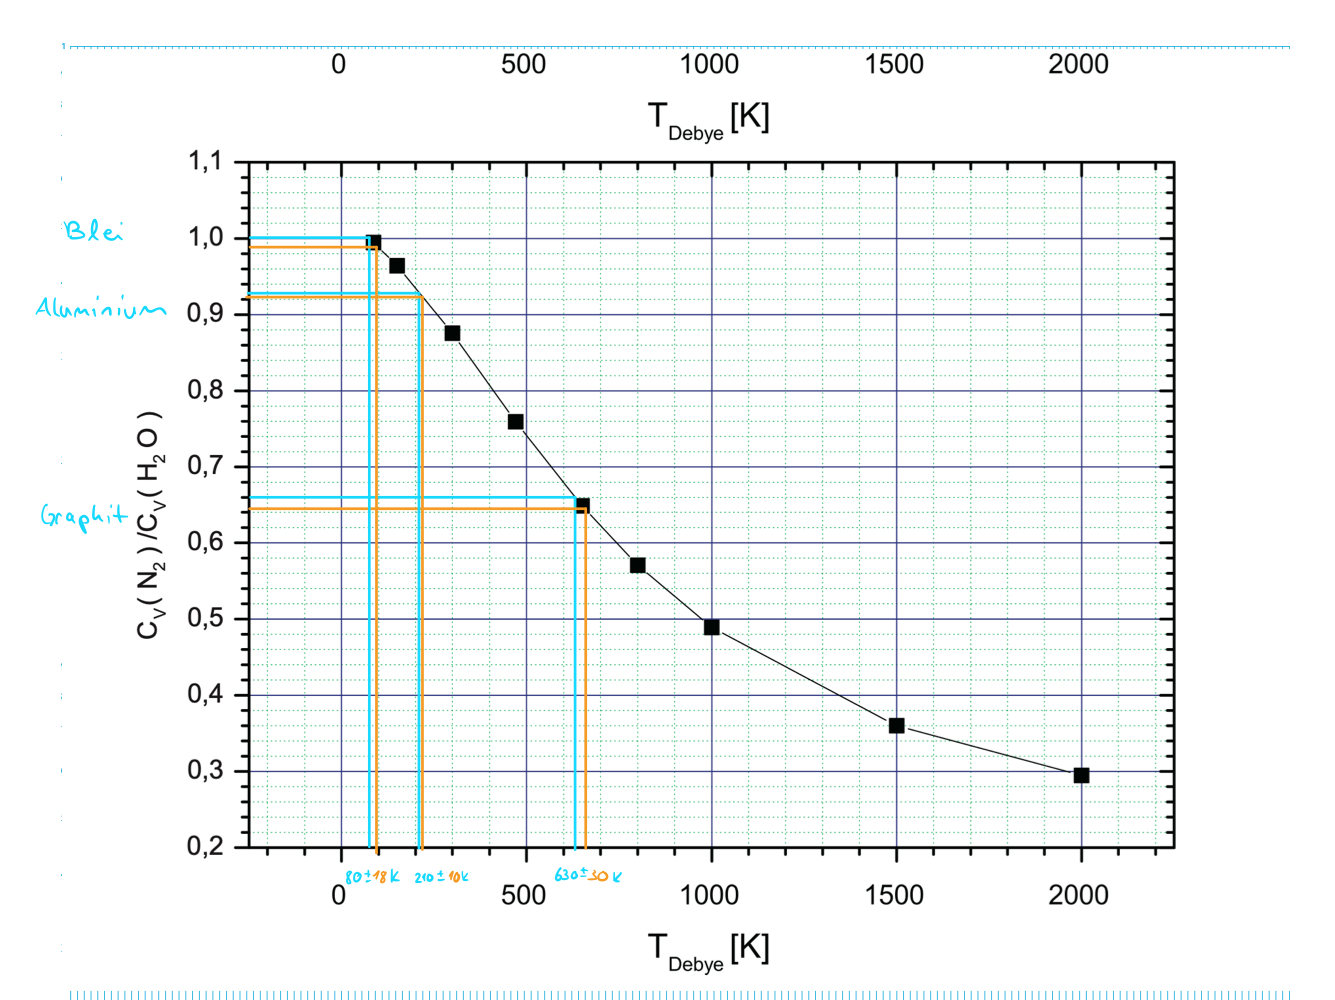
\includegraphics[width=0.95\textwidth,]{Versuch42Dia2.jpeg}
    \caption{Diagramm 2}
\end{figure}
\newpage